\documentclass[a4paper, 11pt]{report}

\usepackage[utf8]{inputenc}
\usepackage[francais]{babel}
\usepackage[T1]{fontenc}
\usepackage{pdfpages}
\usepackage{graphicx}
\usepackage{parskip}
\usepackage{epstopdf}
\DeclareGraphicsRule{.eps}{pdf}{.pdf}{`epstopdf #1}
\pdfcompresslevel=9
\setlength{\parindent}{0.7cm}

\title{Stage de 5ème année\\ \large Rapport intermédiare}
\author{Guillaume Delamare}
\date{\today}

\begin{document}
\renewcommand{\labelitemi}{$\bullet$}
\renewcommand{\labelitemii}{$\diamond$}
\renewcommand{\labelitemiii}{$\ast$}
\renewcommand{\labelitemiv}{$\cdot$}

\maketitle

\section*{Remerciements}
Je tiens, tout d'abords, à remercier mon tuteur, Thomas Ledoux, pour m'avoir offert l'opportunité de travailler au sein de l'équipe ASCOLA. Je le remercie d'autant plus pour l'apport d'expérience et la richesse des situations dans lesquels il me permet de travailler.

Je souhaite ensuite remercier Rémi Sharrock, pour sa bonne humeur et son aide précieuse tout au long de mon travail, ainsi que, l'ensemble des membres de l'équipe ASCOLA et du département d'informatique de l'école des mines de Nantes pour leurs accueils, leurs aides et leurs conseils.

Je remercie aussi mon encadrant, Benoit Parrain, pour l'aide et le suivi tout au long de cet exercice qu'est le stage de fin d'étude. Et pour finir je souhaite remercier Polytech Nantes, dans son ensemble, pour les trois années de formation et d'encadrement dont j'ai pu profiter.


\newpage

\tableofcontents



\chapter{Introduction}
Ce document est un rapport de stage intermédiaire. Je le rédige dans le cadre de mon stage de fin d'étude en cinquième année d'école d'ingénieur à Polytech Nantes. Comme je viens de le dire il s'agit d'un document intermédiaire qui sera complété à la fin de mon stage. 

Ce document est découpé en trois parties. Dans la première je présenterais le contexte de mon stage. Plus précisément, je présenterais le lieu dans lequel se déroule mon stage, puis je parlerais du sujet sur lequel je suis amené à travailler pendant cinq mois.

Dans la deuxième partie je ferais un état de l'art de mon sujet de stage dans lequel je tenterais de définir les notions essentiels à la résolution du problème qu'il m'est posé.

Enfin dans la troisième partie je parlerais des contributions que je propose de réaliser durant mon stage. Ce sera donc le chapitre présentant des parties de mon travail que, lors de la rédaction de ce rapport, j'ai soit déjà effectué, soit que j'effectuerais d'ici la fin de mon stage.

\chapter{Contexte du stage}
\section{Présentation du lieu de stage}
Mon stage de cinquième année se déroule au sein de l’équipe ASCOLA du laboratoire LINA dans les locaux de l’école des Mines de Nantes.
\subsection{L'école des Mines de Nantes}
L’école des Mines de Nantes (EMN) est une école d’ingénieur française sous tutelle du ministère de l’industrie. L’école est rattachée à l’institut Mines-Télécom, au Groupe des écoles des mines et à la Conférence des grandes écoles.

Elle a été créée en 1990 sur le site de la chantrerie à Nantes et accueille 850 élèves ingénieurs en formation initiale. Le recrutement est effectué par concours après deux années de classe préparatoire. En 2011, l’EMN a décerné 250 diplômes d’ingénieur.

L’école est séparée en 5 départements axé sur les thématiques des équipes de recherche de l'école. On dénombre les départements :
\begin{itemize}
	\item D'informatique
	\item D'automatique et productique (DAP)
	\item De systèmes énergétiques et environnement (DSEE)
	\item De physique subatomique et technologies associées (Subatech)
	\item De sciences sociales et de gestion (DSSG)
\end{itemize}

\subsection{L'équipe de Recherche}
Mon stage se déroule dans l'équipe ASCOLA. Cette équipe est installée au sein du département informatique de l’EMN au côté de l'équipe TASK. L'équipe ASCOLA fait partie du LINA (Laboratoire d'Informatique de Nantes Atlantique) ainsi que de l'INRIA (Institut National de Recherche en Informatique et en Automatique).

Cette équipe regroupe une trentaine de personnes qui travaillent sur les langages d'aspects et de composition. Les axes de recherche, tel qu'ils le sont présentés sur la page dédié à l'équipe ASCOLA sur le site de l'INRIA\footnote{http://www.inria.fr/equipes/ascola}, sont :
\begin{itemize}
	\item le développement de nouveaux concepts, de support linguistique, et d'outils pour les applications distribuées permettant de gérer notamment les préoccupations transverses comme la distribution elle-même, les comportements transactionnels et la sécurité ;
	\item la définition d'un modèle qui intègre de manière transparente composants et aspects, en particulier au travers d'une notion d'interface rendant possible le découplage des composants et des aspects concrets, tout en permettant l'analyse et l'application de propriétés de composition dans un contexte hybride composant/aspect ;
	\item l'investigation des relations entre langages dédiés, langages d'aspects et langages de composition. Nous comptons exploiter les similitudes entre ces classes de langages dans le cadre du développement de techniques de conception et d'implémentation des langages de manière à faciliter un développement par transformations d'applications efficaces et correctes à partir d'abstraction de programmation de haut niveau ;
	\item l'étude des fondements de la programmation par aspects et de leurs propriétés de composition au moyen de sémantiques formelles pour les aspects (et les composants) ainsi que des techniques d'analyse, de vérification et de validation correspondantes.
\end{itemize}

Mon stage se déroule sous la tutelle de Thomas Ledoux qui, avec Jean Marc Menaud, Adrien Lèbre, Rémi Sharrock, ainsi que leurs doctorants, travaille sur des aspects cloud computing, virtualisation et écologie des systèmes d'informations.

\section{Présentation du sujet de stage}
Dans cette partie je vais décrire ce qu'est dans la pratique mon sujet de stage. Je joins en annexe le document original de sujet de stage tel qu'il été écrit au moment de la signature de ma convention.

\subsection{Contexte}
Mon stage se positionne dans les travaux GreenIT de l’équipe ASCOLA. Je travaille donc principalement avec la sous-partie de l'équipe qui effectue de la recherche dans ce domaine là.


\subsection{Sujet}
De nos jour, l'informatique est omniprésent. Que ce soit au travail, à la maison, dans nos manières de nous documenté comme dans nos façons de produire, nous utilisons l'outil informatique. Cette informatique est devenu au fil des années de plus en plus gourmande en énergie. La multiplication des réseaux, des centres de données, des terminaux pour se raccorder au système, tout ceci demande toujours plus d'énergie.

Actuellement des efforts sont fait pour optimiser la couche matérielle afin de la rendre toujours plus efficace. Seulement ce n'est pas suffisant. Afin de limiter l'augmentation certaine de la consommation d'énergie des équipements informatique, il faut aussi s'attaquer à la source de ce besoin d'énergie, le logiciel. C'est lui, en effet qui a besoin d'effectuer des calcule, des entrées/sorties, des communications réseaux qui font consommer le matériel.

Des travaux ont bien mis en évidence que, les choix fait lors de la conception d'un logiciel, peuvent être déterminant par rapport à la consommation de celui ci. Ces choix sont divers et variés. Il peut s'agir de la technologie utilisé, mais aussi de l'architecture choisie pour le logiciel ou encore de l'environnement dans lequel ce logiciel fonctionne.

Le sujet de ce stage est donc de proposer, d'étudier et de valider par l'expériementation un certain nombre de suggestions qui permettraient de réduire l'emprunte énergétique d'un logiciel.

\subsection{Objectifs}
Le Sujet de mon stage est donc l'éco-conception de logiciel. Il s'agit d'étudier les différentes pistes qui s'ouvrent à nous pour rendre plus écologique les systèmes d'informations en jouant sur la composante logicielle de ceci. Mon travail est donc de plusieurs ordres.

Je dois tout d'abords rechercher les travaux existants dans ce domaine, qu'il soit centré sur l'éco-conception ou bien positionné sur des domaines anexes comme l'analyse de codes ou bien le cycle de vie du logiciel. Suite à ça, je devrais élaborer un certain nombre de propositions de contribution afin de centrer mon travail à venir. Enfin je devrais expérimenter et valider mes résultats afin de pouvoir emmètre des recommandations en terme d'éco-conception.

Deux travaux transversaux sont à effectuer. Premièrement je dois étudier et mettre en place une méthodologie permettant d'évaluer l'efficacité énergétique d'un code.

\chapter{État de l'art}
\section{Introduction}
\subsection{Portée de l'éco-conception}
L’un des objectifs du Green IT est de réduire l’emprunte énergétique des systèmes d’informations (SI). Cet objectif a déjà été visé dans des travaux sur l'optimisation de la couche matérielle. Dans ce projet, nous souhaitons apporter un nouveau regard en étudiant l’impact du logiciel dans la consommation.

La réduction de l’emprunte énergétique peut être vu de plusieurs façons, qui sont autant d’objectifs intermédiaires pour notre projet :
\begin{itemize}
	\item Baisse de la consommation d’énergie
	\item Allongement de la durée de vie du matériel
	\item Augmentation de l’autonomie des appareils mobiles
\end{itemize}

L’éco-conception de logiciel consiste donc à travailler sur la composante logiciel afin d’améliorer ces critères.

\subsection{Qu'est ce qu'un code gourmand ?}
Répondre à cette question représente déjà une grande partie du travail de ce projet. Dans le cadre de ce projet nous souhaiterions parler de code gourmand au sens énergétique. Un parallèle est à faire avec la gourmandise d’un logiciel au sens efficacité. Cependant, tout code efficace n’est pas forcement optimisé pour une faible consommation énergétique.

La définition d’un code gourmand est loin d’être trivial. En effet, la consommation d’un code est fortement lié à la tâche pour laquelle il a été programmé. Un code servant à décoder un flux vidéo sera, énergétiquement, plus gourmand qu’un code servant à faire une addition. Cette exemple est extrême, mais il montre bien qu’on peut difficilement comparer la gourmandise d’un code à un autre.

En plus de cette difficulté, nous souhaitons voir l'ensemble de l'emprunte énergétique d'un logiciel. Pas seulement la consommation d'électricité lors de son utilisation, mais bien celle tout au long de son cycle de vie.

\subsection{Annalyse du cycle de vie}
L'analyse du cycle de vie (ACV) est un outil utilisé dans l'industrie pour mesurer l'emprunte écologique d'un produit. Il se base sur le cycle de vie du produit de sa conception à sa mise en déchet en passant par sa fabrication et son utilisation. On utilise ensuite un modèle pour transposer ces étapes en un impact environnementaux.

À ma connaissance, il n'existe pas actuellement de modèle permettant d'appliquer l'ACV au logiciel. Cependant, la littérature présente différents points de vue sur le sujet qui peuvent être utilisés comme ébauche à la réalisation d'une ACV logiciel.

\section{Comment juger de l'éco-conception d'un logiciel}
Dans cette section je vais parler de mes recherches dans les outils d'évaluations de l'emprunte énergétique. Je commence par les outils de relevé de consommation à l'exécution d'un système d'information.

\subsection{Mesure de la consommation d'un logiciel}
\subsubsection{Ptop}
pTop est un programme de collecte d’information sur l'exécution de processus sous linux. Il est censé récupérer les données sur l'utilisation du CPU, de la RAM et des échange réseaux. Il doit ensuite être capable, une fois le modèle paramétré, sortir des informations sur la consommation énergétique.

Malheureusement, il s'est avéré que pTop ne fonctionne pas entièrement. Après plusieurs essais infructueux, j'ai supposé que le logiciel avait été abandonné sans être finit.

\paragraph{Procédure d'installation}
\begin{itemize}
    \item récupérer les sources sur http://mist.cs.wayne.edu/ptop.html
    \item installation du nécessaire pour compiler les sources (paquets debian) :
    \begin{itemize}
	\item build-essential
	\item libmysqlclient-dev
	\item libncurses-dev
    \end{itemize}
    \item Installation de la base de données Mysql :
    \begin{itemize}
	\item création d’une base de donées ptop
	\item exécution du script db\_schema.sql
	\item remplacement du login et password pour accéder à la base de données dans le fichier database.c
    \end{itemize}
    \item Compilation :
\end{itemize}

\begin{verbatim}
	# make
	# chmod +x ptop
\end{verbatim}

\paragraph{Exécution}
Lancer le programme au moyen de la commande :

\begin{verbatim}
# ./ptop
\end{verbatim}

Le programme va s'initialiser et enregistrer les mesures dans les bases de données. Il faut ensuite interrompre les mesures au moyen du signal SIGINT.

\paragraph{Données de sortie}
Il n’existe pas, à ma connaissance, de documentation précise sur les données de sortie du programme pTop.  Le programme stock les données dans une base de données Mysql nommé ptop. Elle est composée de quatre tables :
\begin{itemize}
	\item device\_energy
	\item process\_energy
	\item process\_info
	\item sys\_info
\end{itemize}

Seul les deux dernières tables sont remplies par le programme (à cause soit d’un bug, soit d’une version non finit du programme).

\subsubsection{Energy Checker}
Le projet Energy Checker développé par Intel, est un ensemble d’outil destiné à faciliter la remontée et l’affichage des mesures faites sur la consommation d’un programme. Il se compose principalement de l’API energy checker qui permet d’utiliser les mécanismes de remonter d’information (PL - Productivity Link)

\subsubsection{ClassMexer}
ClassMexer est un API java permettant d’estimer la taille en mémoire d’un objet java. On peut télécharger cet API sous la forme d’un fichier JAR à cette adresse : http://www.javamex.com/classmexer/. ClassMexer est un Instrumentation agent comme spécifié dans le pattern Instrument. Cela implique de travailler avec, au minimum, la version 5 de java.

\paragraph{procédure d'installation}
\begin{itemize}
	\item Télécharger l’API
	\item Importer le fichier JAR dans le projet.
	\item Insérer des appels sur l’objet que l’on souhaite mesurer. Par exemple :
\begin{verbatim}
public class Main {
	public static void main(String[] args) {
		String str = "Hello world !";
		
		long noBytes = MemoryUtil.deepMemoryUsageOf(str);
		
		System.out.println(noBytes);
	}
}
\end{verbatim}
	\item Exécuter le programme avec l’option -javaagent:<fichier JAR>
\end{itemize}

\subsubsection{JouleMeter}
Joulemeter est un outil développé par microsoft et qui sert à mesurer la consommation d’énergie sur un ordinateur. Il ne fonctionne que sous Windows 7.

\paragraph{Procédure d'installation}
\begin{itemize}
	\item Télécharger le logiciel sur ce site : Joulemeter
	\item Exécuter le programme.
\end{itemize}

\paragraph{Fonctionnement}
Joulemeter est un logiciel de mesure qui se base sur un modèle de consommation. La première étape est donc de générer ce modèle. Deux méthodes existent.

La première n’est utilisable que sur un ordinateur portable muni d’une batterie. Il suffit de débrancher l’alimentation et de lancer la calibration (15 minuntes sans utiliser le PC). Avant de lancer la calibration, il faut faire attention à arrêter toutes les application afin que le logiciel puisse déterminer une consommation minimum en mode "Idle".

Le deuxième mode nécessite un Wattmètre WattsUp pour générer le modèle. Il suffit de le brancher en USB, de couper toutes les applications possible et de lancer la calibration (3 minutes sans utiliser le PC).

\subsubsection{PowerAPI}
PowerAPI est un outil sur lequel travail l'équipe ADAM de l'université de Lille. Il n'a pas encore été rendu disponible, je n'ai donc pas pu le tester. Les premiers résultat de cet outil ont été présentés lors d'une conférence\footnote{Les documents en lien avec cette conférence ont disparu du site de http://www.inria.fr/centre/grenoble/innovation/rii-snee/demos/powerapi-un-outil-pour-le-diagnostic-energetique-des-logiciels} et parraissent plutot encourageant.

Selon la présentation qui en a été faite, il fonctionne actuellement pour la consommation CPU. Cet outil collecte le temps CPU d'un processus et la fréquence de celui-ci en temps réel. Puis il détermine l'énergie consommée grâce à des tables de consommations par rapport à la fréquence fournis par les fabriquant de processeur.

Cet outil, une fois abouti, devrait vraisemblablement être mis à disposition.


\subsection{Métriques}
Cette partie de l'état de l'art n'est à l'heure actuelle qu'une ébauche. Cela est dù à ma découverte récemment de nouvelles informations qui nécessite un travail de lecture que je n'ai pas encore eu le temps de faire.

Les métriques que je souhaite présenté sont utilisés pour juger l'efficacité énergétique d'installation informatique comme les centres de données. Mes recherches bibliographiques m'ont amené à en distinguer trois intéressantes :
\begin{itemize}
	\item PUE (Power Usage Effectiveness)
	\item ERE (Energy Reuse Effectiveness) (ref)
	\item CUE (Carbon Usage Effectiveness)
\end{itemize}

L’indice PUE met en valeur la perte énergétique des équipements. Il ne prend pas en compte la valorisation de ces pertes. C'est l'indice utilisé comme référence depuis des années. Les deux autres indices sont nouveau et propose des ajout intéressant par rapport au PUE. L’indice ERE essai de rattraper les faiblesses du PUE en prenant en compte la revalorisation. L’indice CUE permet de valoriser le type d’énergie utilisée.

Je souhaite les présenter plus en détail dans la prochaine version de ce document, car ce son des outils qui mettent en évidence le fait qu'une application ne consomme pas uniquement ce qu'elle à besoin pour faire ses calcule  et donc ils mettent en évidence l'importance du cycle de vie dans l'éco-conception.

\section{Bonnes pratiques et patrons de conception}
\subsection{Modularité}
Décrire les différence entre programme Monolithique et programme modulaire
	Liens avec les OS (Monolithique Vs Micro noyau)
	Linux serait monolythique au sens OS mais modulaire au sens logiciel ?

POO = modulaire ?
	Si oui qu’est ce qu’est OSGi
	Début de réponse : OSGi = approche Objet au niveau architecture logiciel

Question de la compatibilité inter-langage des modules. Comment rendre modulaire un programme au point qu’il fonctionne de la même façon quelque soit les langage d’origine de ses module.

Qu’est ce qu’un module en théorie ?
\begin{figure}
	\begin{center}
		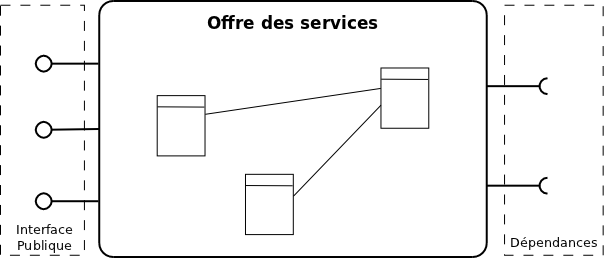
\includegraphics[width=300px]{../../Figures/Bibliographie/modular}
		\caption{Repsésentation d'un module}
	\end{center}
\end{figure}

\begin{itemize}
	\item Cohérence des services offert dans un module. -> éviter de faire une boite à outils pour tout faire.
	\item Offre ses services au travers d’une interface public.
	\item Privilégié l’utilisation/dépendance à d’autre module plutôt que l’encapsulation ou la réécriture au sein du module.
	\item Un module qui fournis un service peut être remplacé par un autre module qui fournis le même service.
\end{itemize}
\subsection{OSGi}
modularité de code = activation ou désactivation de module. Cela libère de la ressource mais implique certainement une contrepartie : par exemple des accès disque multiplié pour activer un module.

OSGI est une spécification, élaboré par l’OSGi Alliance (http://www.osgi.org), qui a pour but de décrire un framework pour rendre les applications Java modulaire. Différentes implémentations de ce framework ont été développés à partir de cette spécification. Les plus connu sont Equinox développé par l’équipe du projet eclipse, Felix issu du projet universitaire Oscar et maintenu par apache ou encore Knopflerfish élaboré par MakeWave.
\section{Conclusion}

\chapter{Proposition de contributions}
\section{Introduction}
Dans ce chapitre, je vais détailler sous la forme d'un plan commenté, le contenu du travail que je souhaite effectuer. Certaine de ces contributions sont déjà passé, d'autre sont en cours enfin, d'autre sont encore à réaliser. Dans le cadre de ce rapport intermédiaire, je ne détaillerais pas les résultats obtenu jusque là. Cela fera l'objet d'un autre chapitre dans le rapport final.

\section{Mesure de Consommation}
Cet ensemble de contribution concerne l'évaluation de la de la consommation d'un logiciel en fonctionnement. Cette étude permettra, par la suite, d'évaluer la pertinence et la validité des solutions proposées pour éco-concevoir des logiciels. L'objectif est d'obtenir une méthode fiable pour mesurer les avantages et les inconvénients (d'un point de vue énergétique) de certaines techniques ou technologies.

Afin d'obtenir les résultats les plus fiables, je propose d'étudier plusieurs systèmes de mesure. En particulier confronter la grossièreté de la mesure par wattmètre à l'approximation de la mesure par modèle de consommation (par exemple JouleMetter) et d'en étudier la complémentarité.

Cette partie des contributions prendra donc la forme de testes sur lesquels on enregistrera les résultats pour les analyser et essayer d'en tirer le meilleur résultat possible.

\section{Langage et algorithmique}
Dans cette partie je souhaite réaliser un certain nombre de petits programmes qui permettraient, pour chacun, de mettre en valeur une bonne pratique de programmation. L'objectif est, à chaque fois, de cibler un critère particulier sur un langage donné. Ces programmes permettront d'effectuer des expérimentations ainsi que des démonstrations de la validité de ce que l'on propose pour éco-concevoir les logiciels.

Dans un deuxième temps, je pense utiliser des outils d'analyses de code comme le plugin eclipse FindBug afin de mettre en place des règles identifié et expérimenté dans les programmes décrit ci-dessus. Cela permettra d'illustrer la facilité de corriger le code énergivore de manière automatique du moment que l'on a identifié ce code.

Enfin, dans une dernière partie plus orientée sur l'algorithmique, je propose de réaliser un programme basé sur des algorithmes de trie que l'on pourra faire tourner en continu. Ces algorithmes seront, en plus, paramétrable (par exemple des temps de pause entre chaque étape) afin de mesurer l'impact de différentes stratégies sur un même traitement qui est le tri.

\section{Architecture logicielle}
Dans mes contributions, je souhaite travailler sur l'architecture logicielle en évaluant l'intérêt que peut avoir la programmation modulaire sur la consommation d'énergie. Pour cela je propose de réflechir et de développer un prototype, basé sur la technologie OSGi, permettant de charger et décharger les différentes fonctionnalités d'un logiciel au fur et à mesure que l'utilisateur se sert du logiciel.

\begin{figure}
    \begin{center}
	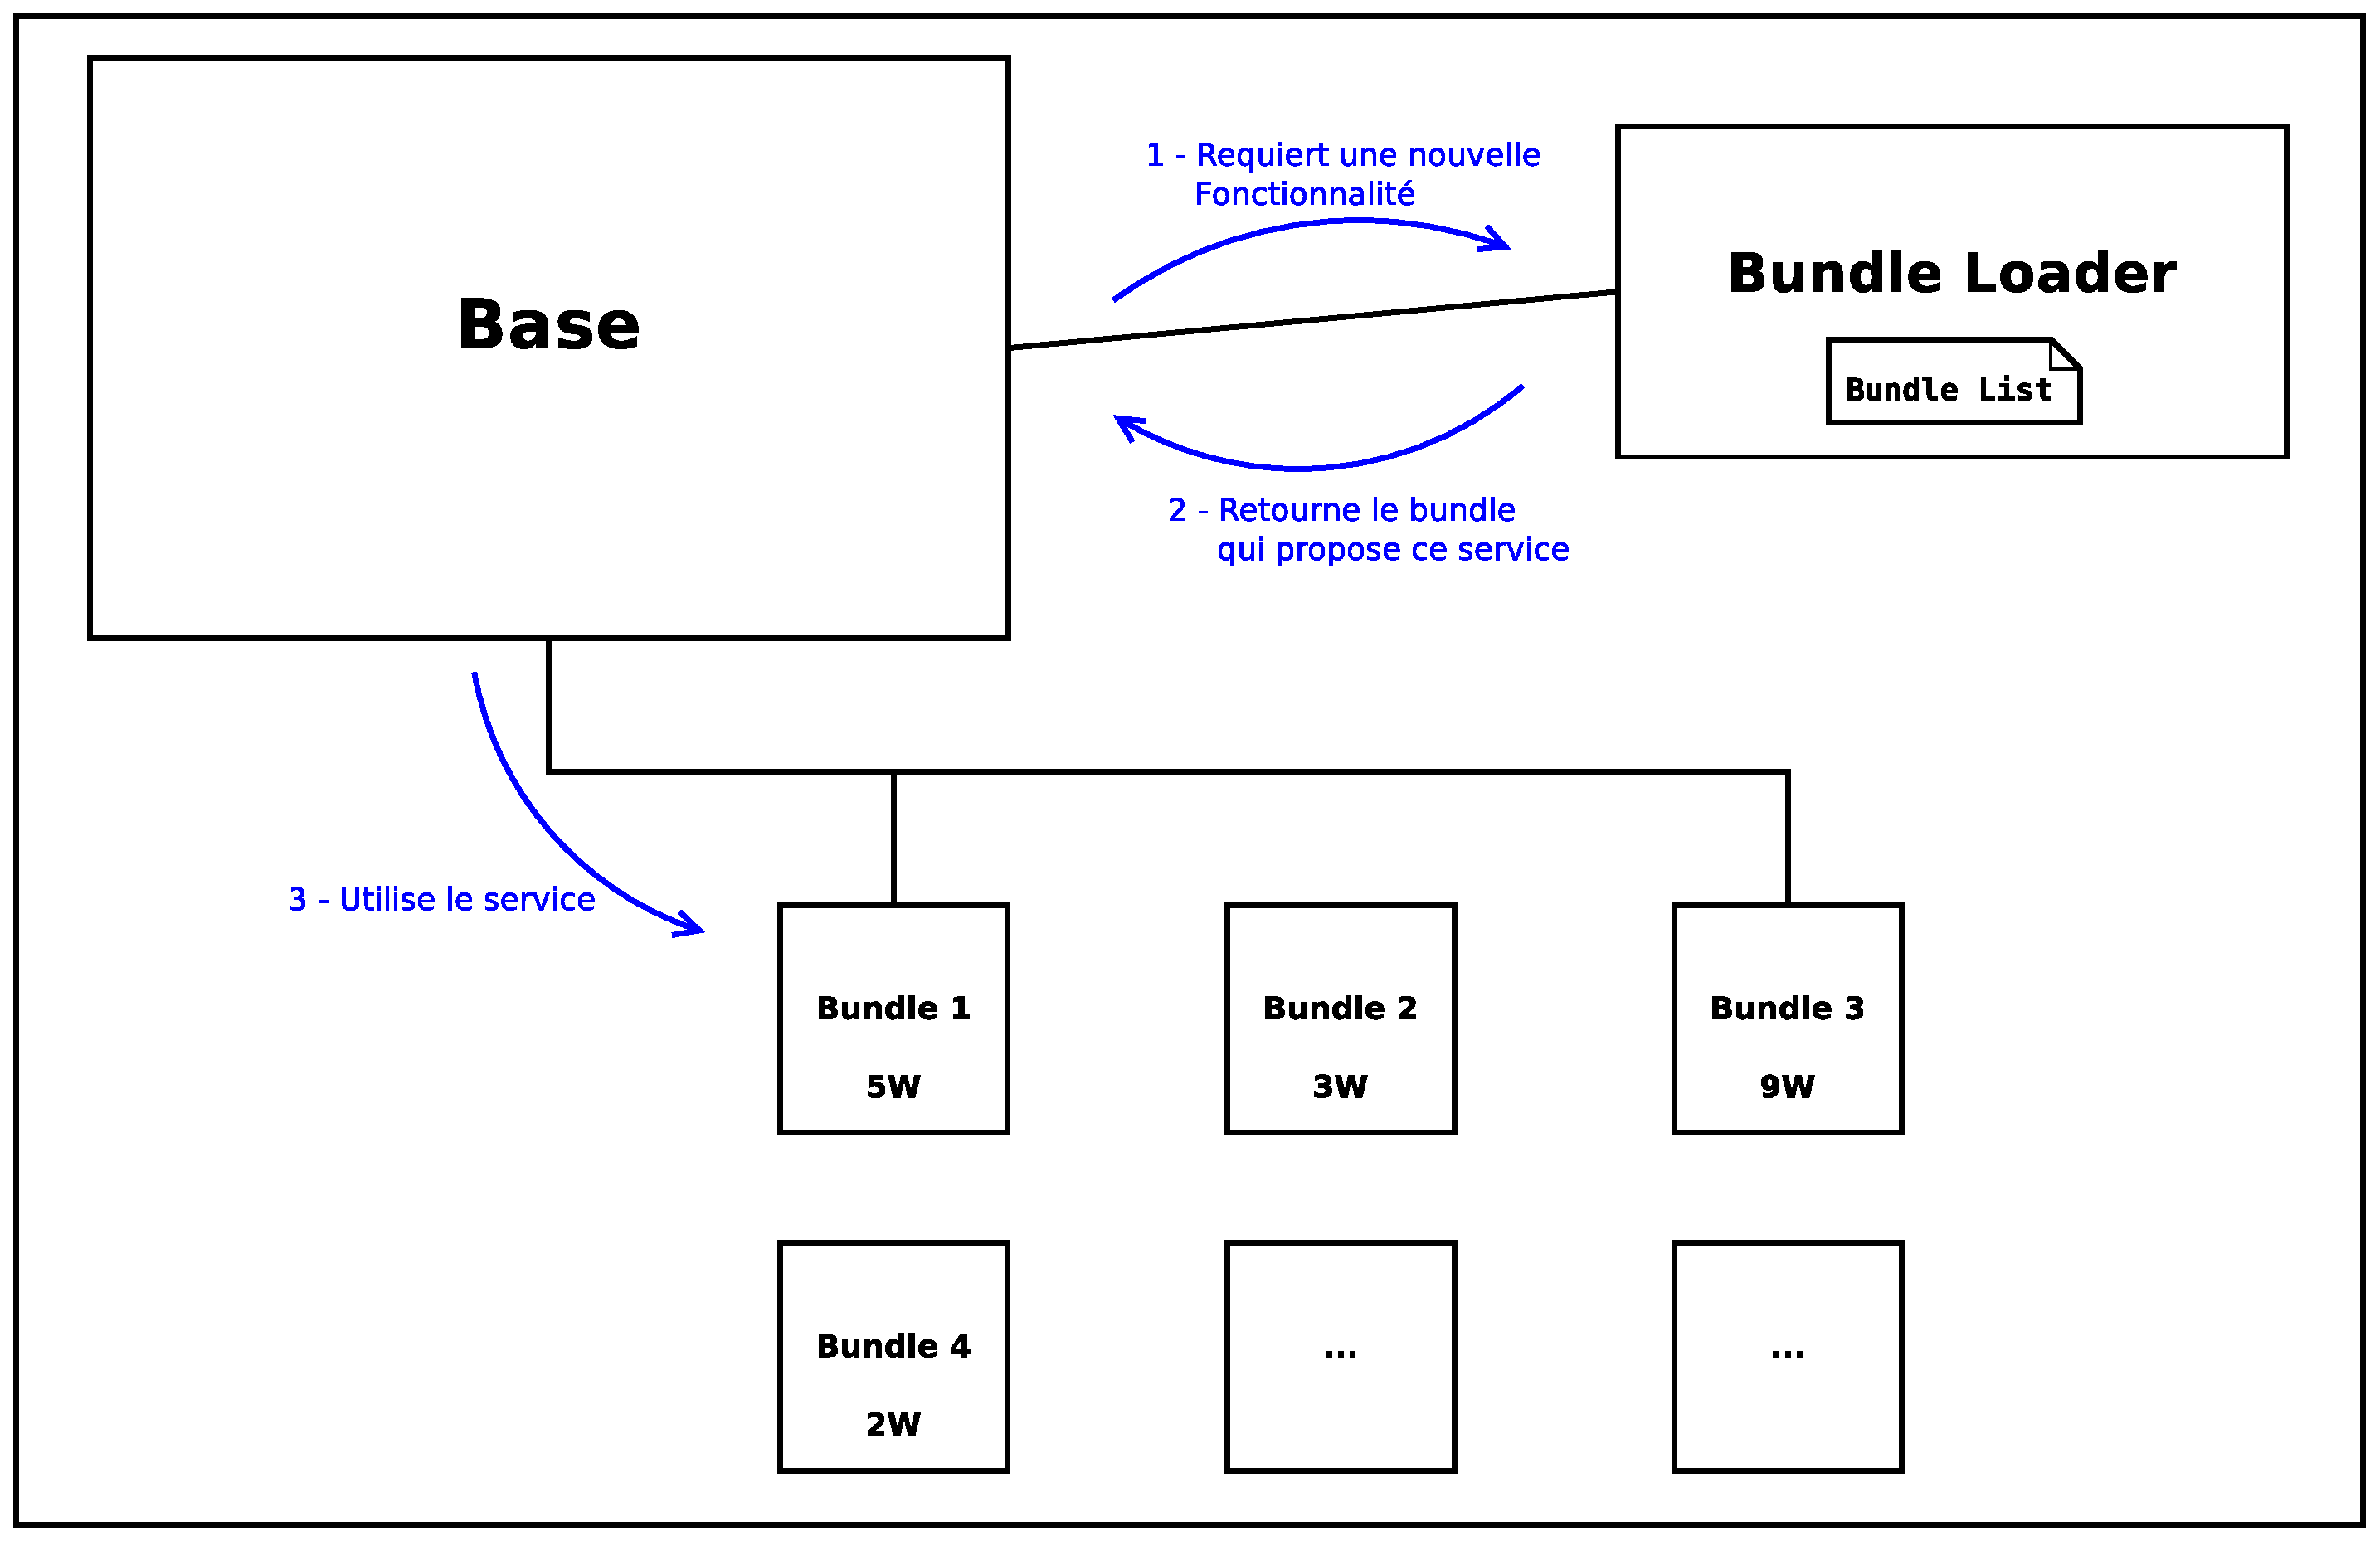
\includegraphics[width=300pt]{../../Figures/OSGi/EcoPattern_General_Figure}
	\caption{Prototype d'application modulaire - Schéma général}
    \end{center}
\end{figure}

Une autre possibilité de contribution dans le domaine de l'architecture logicielle serait de travailler sur le niveau de service fournit par une application. Par exemple un service web qui se dégrade en fonction des contraintes énergétique qui lui sont imposés. La dégradation serait de ne pas renvoyer l'ensemble des résultats à une requête ou bien de ne plus envoyer que le texte, mais pas les images associées.

\chapter{Conclusion}
Comme on vient de le voir dans le dernier chapitre, l'éco-conception est un sujet vaste qui demandera plus de travail que celui que l'on peut mener tout au long d'un stage de cinq mois. Il y a beaucoup de domaine qui ne sont pas abordés dans ce rapport et qui ne pourront, peut être pas, l'être lors de la version finale. Néanmoins, j'essaie de proposer une vision large des possibilités que peuvent nous offrir un travail de réflection sur la manière de rendre plus écologique nos logiciels.

La suite du travail est toute faite, il s'agit maintenant de développer toutes ces idées et de les critiquer afin d'obtenir une des résultats intéressants qui permettront peut être de poursuivre le travail dans ce domaine.

\listoffigures{}
\listoftables{}
\appendix

\chapter{Sujet de stage}
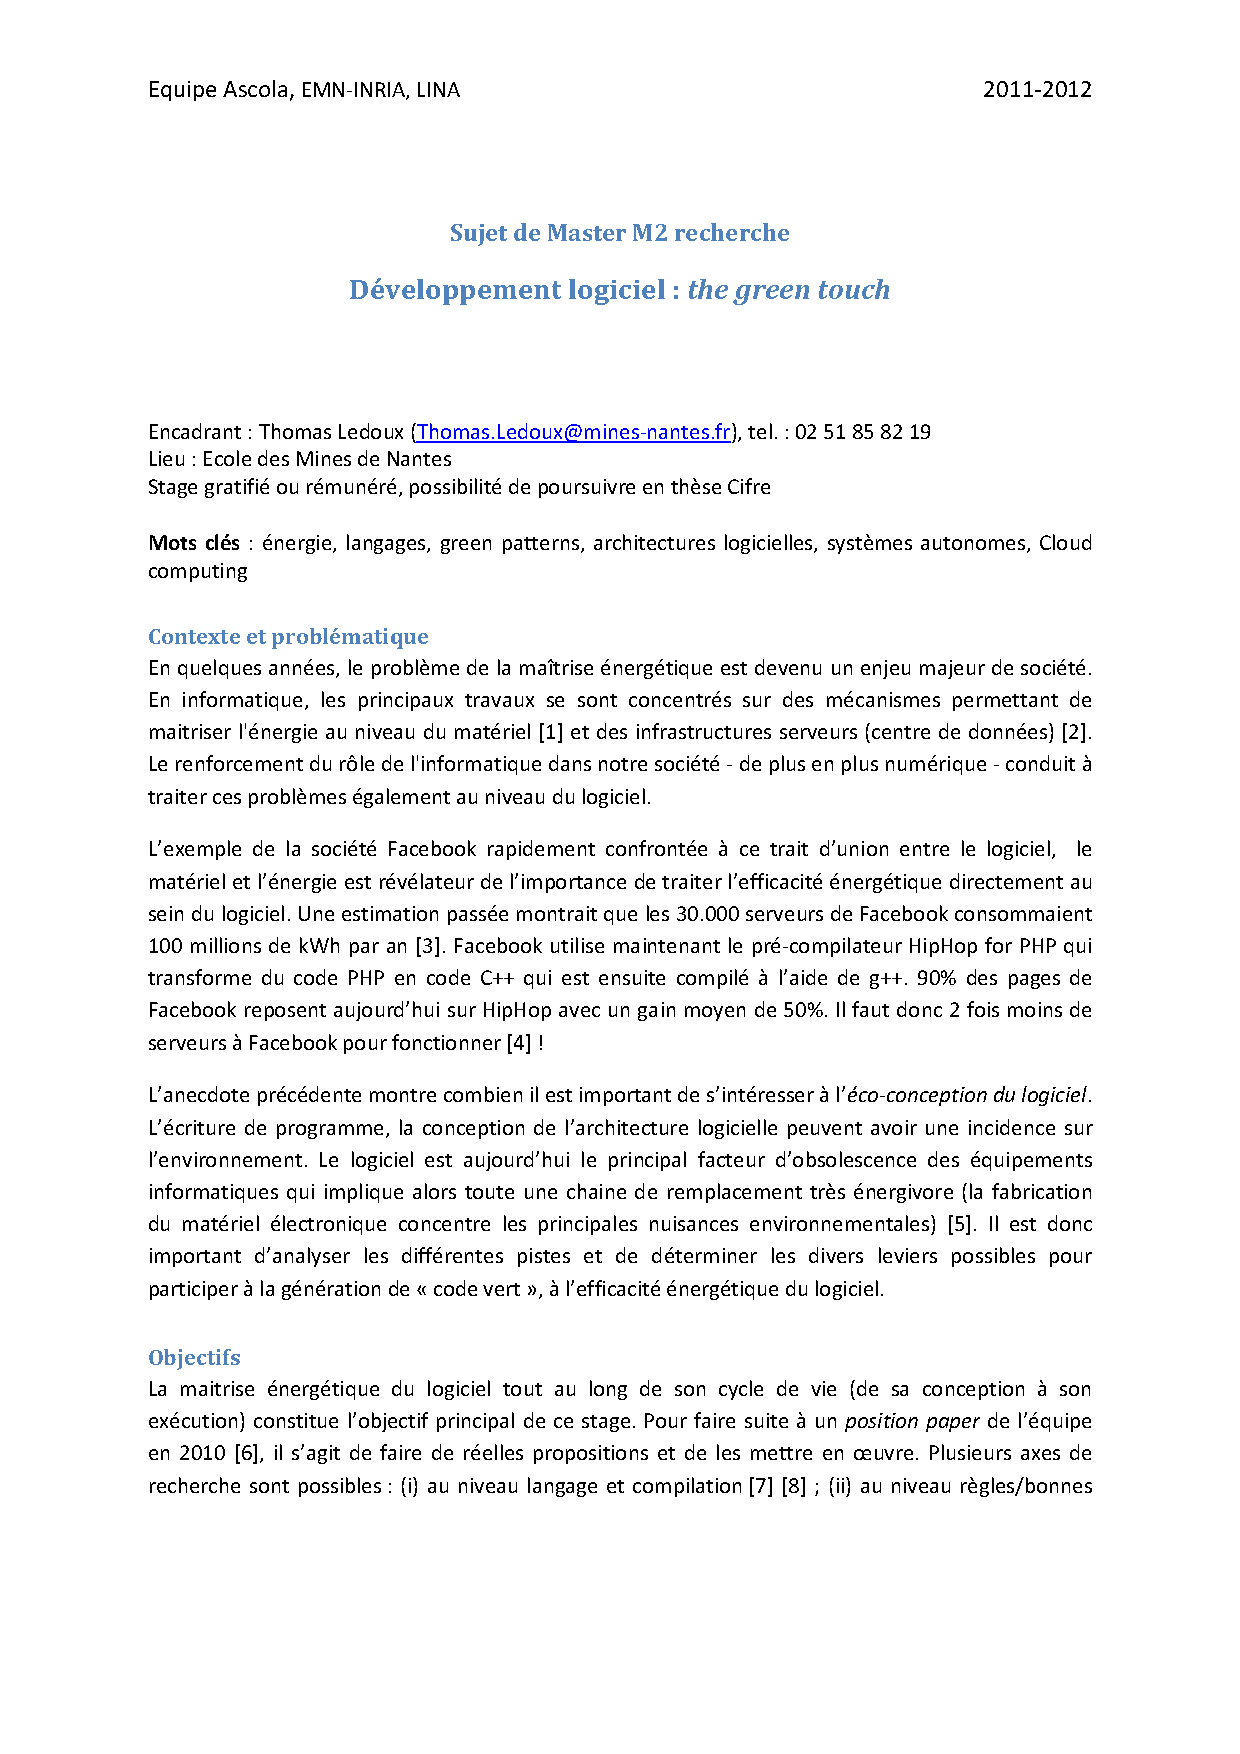
\includepdf[pages=-]{../../Documents/Sujet_Master_EcoConceptionGL.pdf}


\end{document}
